%% bare_conf.tex
%% V1.4b
%% 2015/08/26
%% by Michael Shell
%% See:
%% http://www.michaelshell.org/
%% for current contact information.
%%
%% This is a skeleton file demonstrating the use of IEEEtran.cls
%% (requires IEEEtran.cls version 1.8b or later) with an IEEE
%% conference paper.
%%
%% Support sites:
%% http://www.michaelshell.org/tex/ieeetran/
%% http://www.ctan.org/pkg/ieeetran
%% and
%% http://www.ieee.org/

%%*************************************************************************
%% Legal Notice:
%% This code is offered as-is without any warranty either expressed or
%% implied; without even the implied warranty of MERCHANTABILITY or
%% FITNESS FOR A PARTICULAR PURPOSE! 
%% User assumes all risk.
%% In no event shall the IEEE or any contributor to this code be liable for
%% any damages or losses, including, but not limited to, incidental,
%% consequential, or any other damages, resulting from the use or misuse
%% of any information contained here.
%%
%% All comments are the opinions of their respective authors and are not
%% necessarily endorsed by the IEEE.
%%
%% This work is distributed under the LaTeX Project Public License (LPPL)
%% ( http://www.latex-project.org/ ) version 1.3, and may be freely used,
%% distributed and modified. A copy of the LPPL, version 1.3, is included
%% in the base LaTeX documentation of all distributions of LaTeX released
%% 2003/12/01 or later.
%% Retain all contribution notices and credits.
%% ** Modified files should be clearly indicated as such, including  **
%% ** renaming them and changing author support contact information. **
%%*************************************************************************


% *** Authors should verify (and, if needed, correct) their LaTeX system  ***
% *** with the testflow diagnostic prior to trusting their LaTeX platform ***
% *** with production work. The IEEE's font choices and paper sizes can   ***
% *** trigger bugs that do not appear when using other class files.       ***                          ***
% The testflow support page is at:
% http://www.michaelshell.org/tex/testflow/



\documentclass[conference]{IEEEtran}
% Some Computer Society conferences also require the compsoc mode option,
% but others use the standard conference format.
%
% If IEEEtran.cls has not been installed into the LaTeX system files,
% manually specify the path to it like:
% \documentclass[conference]{../sty/IEEEtran}





% Some very useful LaTeX packages include:
% (uncomment the ones you want to load)


% *** MISC UTILITY PACKAGES ***
%
%\usepackage{ifpdf}
% Heiko Oberdiek's ifpdf.sty is very useful if you need conditional
% compilation based on whether the output is pdf or dvi.
% usage:
% \ifpdf
%   % pdf code
% \else
%   % dvi code
% \fi
% The latest version of ifpdf.sty can be obtained from:
% http://www.ctan.org/pkg/ifpdf
% Also, note that IEEEtran.cls V1.7 and later provides a builtin
% \ifCLASSINFOpdf conditional that works the same way.
% When switching from latex to pdflatex and vice-versa, the compiler may
% have to be run twice to clear warning/error messages.






% *** CITATION PACKAGES ***
%
%\usepackage{cite}
% cite.sty was written by Donald Arseneau
% V1.6 and later of IEEEtran pre-defines the format of the cite.sty package
% \cite{} output to follow that of the IEEE. Loading the cite package will
% result in citation numbers being automatically sorted and properly
% "compressed/ranged". e.g., [1], [9], [2], [7], [5], [6] without using
% cite.sty will become [1], [2], [5]--[7], [9] using cite.sty. cite.sty's
% \cite will automatically add leading space, if needed. Use cite.sty's
% noadjust option (cite.sty V3.8 and later) if you want to turn this off
% such as if a citation ever needs to be enclosed in parenthesis.
% cite.sty is already installed on most LaTeX systems. Be sure and use
% version 5.0 (2009-03-20) and later if using hyperref.sty.
% The latest version can be obtained at:
% http://www.ctan.org/pkg/cite
% The documentation is contained in the cite.sty file itself.






% *** GRAPHICS RELATED PACKAGES ***
%
\ifCLASSINFOpdf
   \usepackage[pdftex]{graphicx}
  % declare the path(s) where your graphic files are
  % \graphicspath{{../pdf/}{../jpeg/}}
  % and their extensions so you won't have to specify these with
  % every instance of \includegraphics
  % \DeclareGraphicsExtensions{.pdf,.jpeg,.png}
\else
  % or other class option (dvipsone, dvipdf, if not using dvips). graphicx
  % will default to the driver specified in the system graphics.cfg if no
  % driver is specified.
   \usepackage[dvips]{graphicx}
  % declare the path(s) where your graphic files are
  % \graphicspath{{../eps/}}
  % and their extensions so you won't have to specify these with
  % every instance of \includegraphics
  % \DeclareGraphicsExtensions{.eps}
\fi
% graphicx was written by David Carlisle and Sebastian Rahtz. It is
% required if you want graphics, photos, etc. graphicx.sty is already
% installed on most LaTeX systems. The latest version and documentation
% can be obtained at: 
% http://www.ctan.org/pkg/graphicx
% Another good source of documentation is "Using Imported Graphics in
% LaTeX2e" by Keith Reckdahl which can be found at:
% http://www.ctan.org/pkg/epslatex
%
% latex, and pdflatex in dvi mode, support graphics in encapsulated
% postscript (.eps) format. pdflatex in pdf mode supports graphics
% in .pdf, .jpeg, .png and .mps (metapost) formats. Users should ensure
% that all non-photo figures use a vector format (.eps, .pdf, .mps) and
% not a bitmapped formats (.jpeg, .png). The IEEE frowns on bitmapped formats
% which can result in "jaggedy"/blurry rendering of lines and letters as
% well as large increases in file sizes.
%
% You can find documentation about the pdfTeX application at:
% http://www.tug.org/applications/pdftex





% *** MATH PACKAGES ***
%
\usepackage{amsmath}
% A popular package from the American Mathematical Society that provides
% many useful and powerful commands for dealing with mathematics.
%
% Note that the amsmath package sets \interdisplaylinepenalty to 10000
% thus preventing page breaks from occurring within multiline equations. Use:
%\interdisplaylinepenalty=2500
% after loading amsmath to restore such page breaks as IEEEtran.cls normally
% does. amsmath.sty is already installed on most LaTeX systems. The latest
% version and documentation can be obtained at:
% http://www.ctan.org/pkg/amsmath





% *** SPECIALIZED LIST PACKAGES ***
%
%\usepackage{algorithmic}
% algorithmic.sty was written by Peter Williams and Rogerio Brito.
% This package provides an algorithmic environment fo describing algorithms.
% You can use the algorithmic environment in-text or within a figure
% environment to provide for a floating algorithm. Do NOT use the algorithm
% floating environment provided by algorithm.sty (by the same authors) or
% algorithm2e.sty (by Christophe Fiorio) as the IEEE does not use dedicated
% algorithm float types and packages that provide these will not provide
% correct IEEE style captions. The latest version and documentation of
% algorithmic.sty can be obtained at:
% http://www.ctan.org/pkg/algorithms
% Also of interest may be the (relatively newer and more customizable)
% algorithmicx.sty package by Szasz Janos:
% http://www.ctan.org/pkg/algorithmicx




% *** ALIGNMENT PACKAGES ***
%
%\usepackage{array}
% Frank Mittelbach's and David Carlisle's array.sty patches and improves
% the standard LaTeX2e array and tabular environments to provide better
% appearance and additional user controls. As the default LaTeX2e table
% generation code is lacking to the point of almost being broken with
% respect to the quality of the end results, all users are strongly
% advised to use an enhanced (at the very least that provided by array.sty)
% set of table tools. array.sty is already installed on most systems. The
% latest version and documentation can be obtained at:
% http://www.ctan.org/pkg/array


% IEEEtran contains the IEEEeqnarray family of commands that can be used to
% generate multiline equations as well as matrices, tables, etc., of high
% quality.




% *** SUBFIGURE PACKAGES ***
%\ifCLASSOPTIONcompsoc
%  \usepackage[caption=false,font=normalsize,labelfont=sf,textfont=sf]{subfig}
%\else
%  \usepackage[caption=false,font=footnotesize]{subfig}
%\fi
% subfig.sty, written by Steven Douglas Cochran, is the modern replacement
% for subfigure.sty, the latter of which is no longer maintained and is
% incompatible with some LaTeX packages including fixltx2e. However,
% subfig.sty requires and automatically loads Axel Sommerfeldt's caption.sty
% which will override IEEEtran.cls' handling of captions and this will result
% in non-IEEE style figure/table captions. To prevent this problem, be sure
% and invoke subfig.sty's "caption=false" package option (available since
% subfig.sty version 1.3, 2005/06/28) as this is will preserve IEEEtran.cls
% handling of captions.
% Note that the Computer Society format requires a larger sans serif font
% than the serif footnote size font used in traditional IEEE formatting
% and thus the need to invoke different subfig.sty package options depending
% on whether compsoc mode has been enabled.
%
% The latest version and documentation of subfig.sty can be obtained at:
% http://www.ctan.org/pkg/subfig




% *** FLOAT PACKAGES ***
%
%\usepackage{fixltx2e}
% fixltx2e, the successor to the earlier fix2col.sty, was written by
% Frank Mittelbach and David Carlisle. This package corrects a few problems
% in the LaTeX2e kernel, the most notable of which is that in current
% LaTeX2e releases, the ordering of single and double column floats is not
% guaranteed to be preserved. Thus, an unpatched LaTeX2e can allow a
% single column figure to be placed prior to an earlier double column
% figure.
% Be aware that LaTeX2e kernels dated 2015 and later have fixltx2e.sty's
% corrections already built into the system in which case a warning will
% be issued if an attempt is made to load fixltx2e.sty as it is no longer
% needed.
% The latest version and documentation can be found at:
% http://www.ctan.org/pkg/fixltx2e


\usepackage{stfloats}
% stfloats.sty was written by Sigitas Tolusis. This package gives LaTeX2e
% the ability to do double column floats at the bottom of the page as well
% as the top. (e.g., "\begin{figure*}[!b]" is not normally possible in
% LaTeX2e). It also provides a command:
%\fnbelowfloat
% to enable the placement of footnotes below bottom floats (the standard
% LaTeX2e kernel puts them above bottom floats). This is an invasive package
% which rewrites many portions of the LaTeX2e float routines. It may not work
% with other packages that modify the LaTeX2e float routines. The latest
% version and documentation can be obtained at:
% http://www.ctan.org/pkg/stfloats
% Do not use the stfloats baselinefloat ability as the IEEE does not allow
% \baselineskip to stretch. Authors submitting work to the IEEE should note
% that the IEEE rarely uses double column equations and that authors should try
% to avoid such use. Do not be tempted to use the cuted.sty or midfloat.sty
% packages (also by Sigitas Tolusis) as the IEEE does not format its papers in
% such ways.
% Do not attempt to use stfloats with fixltx2e as they are incompatible.
% Instead, use Morten Hogholm'a dblfloatfix which combines the features
% of both fixltx2e and stfloats:
%
%\usepackage{dblfloatfix}
% The latest version can be found at:
% http://www.ctan.org/pkg/dblfloatfix




% *** PDF, URL AND HYPERLINK PACKAGES ***
%
%\usepackage{url}
% url.sty was written by Donald Arseneau. It provides better support for
% handling and breaking URLs. url.sty is already installed on most LaTeX
% systems. The latest version and documentation can be obtained at:
% http://www.ctan.org/pkg/url
% Basically, \url{my_url_here}.




% *** Do not adjust lengths that control margins, column widths, etc. ***
% *** Do not use packages that alter fonts (such as pslatex).         ***
% There should be no need to do such things with IEEEtran.cls V1.6 and later.
% (Unless specifically asked to do so by the journal or conference you plan
% to submit to, of course. )

\usepackage[english]{babel}
\usepackage{svg}
\usepackage{url} % um URL Links zu zitieren
\usepackage[]{footmisc} % um Footnotes zu machen
\usepackage{xcolor} % um farbigen text zu schreiben

% correct bad hyphenation here
\hyphenation{op-tical net-works semi-conduc-tor}


\usepackage[backend=biber,
style=alphabetic,
]{biblatex}

\addbibresource{bib.tex}


\begin{document}
%
% paper title
% Titles are generally capitalized except for words such as a, an, and, as,
% at, but, by, for, in, nor, of, on, or, the, to and up, which are usually
% not capitalized unless they are the first or last word of the title.
% Linebreaks \\ can be used within to get better formatting as desired.
% Do not put math or special symbols in the title.
\title{A Primer on Anomaly Detection Strategies in Urban Traffic}



% author names and affiliations
% use a multiple column layout for up to three different
% affiliations
\author{\IEEEauthorblockN{Roman Kessler}
\IEEEauthorblockA{University of Applied Sciences Darmstadt\\
roman.kessler@stud.h-da.de}}

% conference papers do not typically use \thanks and this command
% is locked out in conference mode. If really needed, such as for
% the acknowledgment of grants, issue a \IEEEoverridecommandlockouts
% after \documentclass

% for over three affiliations, or if they all won't fit within the width
% of the page, use this alternative format:
% 
%\author{\IEEEauthorblockN{Michael Shell\IEEEauthorrefmark{1},
%Homer Simpson\IEEEauthorrefmark{2},
%James Kirk\IEEEauthorrefmark{3}, 
%Montgomery Scott\IEEEauthorrefmark{3} and
%Eldon Tyrell\IEEEauthorrefmark{4}}
%\IEEEauthorblockA{\IEEEauthorrefmark{1}School of Electrical and Computer Engineering\\
%Georgia Institute of Technology,
%Atlanta, Georgia 30332--0250\\ Email: see http://www.michaelshell.org/contact.html}
%\IEEEauthorblockA{\IEEEauthorrefmark{2}Twentieth Century Fox, Springfield, USA\\
%Email: homer@thesimpsons.com}
%\IEEEauthorblockA{\IEEEauthorrefmark{3}Starfleet Academy, San Francisco, California 96678-2391\\
%Telephone: (800) 555--1212, Fax: (888) 555--1212}
%\IEEEauthorblockA{\IEEEauthorrefmark{4}Tyrell Inc., 123 Replicant Street, Los Angeles, California 90210--4321}}

% use for special paper notices
%\IEEEspecialpapernotice{(Invited Paper)}




% make the title area
\maketitle

% As a general rule, do not put math, special symbols or citations
% in the abstract
%\begin{abstract}
%The abstract goes here.
%\end{abstract}

% no keywords




% For peer review papers, you can put extra information on the cover
% page as needed:
% \ifCLASSOPTIONpeerreview
% \begin{center} \bfseries EDICS Category: 3-BBND \end{center}
% \fi
%
% For peerreview papers, this IEEEtran command inserts a page break and
% creates the second title. It will be ignored for other modes.
\IEEEpeerreviewmaketitle



%-------------------------------
%	CONTENTS
%-------------------------------
\begin{abstract}
    %\textcolor{red}{to do}
    Urban traffic comprises a complex interplay between many agents, such as cars, trucks, and cyclists, which share a mutual infrastructure, i.e. a road network. Further to individual agents, other -- e.g., essential agents from other infrastructures such as emergency or fire brigade -- depend on a flawless operation of the urban traffic infrastructure. When a particular segment of the road network fails, for instance due to traffic accidents or congestion, it may be desired to early recognize such a failure, and to quickly restore the traffic, to prevent downstream infrastructures to be harmed. The first step therefore is to detect a possible failure, i.e. anomaly, forthwith.
    In the present work anomaly detection methods in the context of urban traffic surveillance will be introduced. First, different kinds of anomalies will be characterized, and particular challenges when it comes to anomaly detection will be outlined. Second, different conceptual methods for anomaly detection will be illustrated. The outlined methods were chosen to follow different theoretical approaches. In principle, all of them can be applied to many different anomaly detection use cases. Third, some exemplary studies using variations of the introduced anomaly detection approaches in the context of traffic anomaly detection and forecasting will be introduced. Finally, the present work will propose an integration of those example studies with other methods of anomaly detection and forecasting to motivate future directions in urban traffic anomaly detection. 
\end{abstract}

%\textcolor{red}{Table of contents only provisional, I will delete it in the end}
%\setcounter{tocdepth}{2} % depth of toc
%\tableofcontents

\section{Introduction}

In the last decades, large cities have grown significantly and this development is expected to continue \cite{UN2014Urbanization}. This urbanization is associated with growing traffic infrastructures, which need to be adapted for the changing demands by the rising population counts in such large cities. Meanwhile, progressive digitization can be used to monitor the complex traffic infrastructure \cite{mohammadi2017}. Such monitoring ought to subserve the maintenance of a flawless operation, in particular via early detection of malicious events (i.e., anomaly detection).

At the same time, there also exist high interdependencies between traffic and other critical infrastructures (i.e., sector coupling) \cite{ouyang2014}. For instance, ambulance, police, or fire brigade depend on a smooth operation of a city's traffic infrastructure in emergency cases. On the same time, economy is depending on traffic infrastructure to maintain supply chains. To protect this critical infrastructure digital twins can be deployed \cite{ouyang2014}. Digital twins are artificial replicas of the physical infrastructure, which allow monitoring traffic by the use of real time surveillance \cite{mohammadi2017}. Whereas digital twins in this context might be used to optimize traffic or simulate extreme events (e.g., jams or floods), this paper will focus on possibilities to detect or to forecast such extreme events in an operational setting. Such a real time anomaly detection is critical for local authorities to be capable to react immediately to a disruption. Reaction is either obligatory to prevent the traffic's failure, to bring the system back online rapidly, or to curb downstream negative impacts such as the flawless operation of interdependent infrastructures.

Anomalies may have different sources. On the one hand, the traffic itself can lead to an anomaly such as a spontaneous congestion (i.e., internal). On the other hand, malicious events can be introduced either by purpose, for instance in an act of war or terror, or by force majeure such as extreme weather events (i.e., external).
In both cases, early anomaly detection in traffic infrastructure is crucial to rapidly restore full functionality of the city's traffic, and to prevent downstream critical infrastructures to fail. 
Further, the sensors themselves may either have a technical failure or be victim of attacks. Such events might be represented as anomaly in the data. Therefore, an anomaly or outlier could be a rare behavior within the traffic, a measurement error, a technical defect in the surveillance system, or a reaction of the traffic to an unexpected event.

The present work aims to identify techniques for anomaly detection, and evaluates their suitability for the use within a city's traffic infrastructure. For this aim, I introduce a distinction of techniques. \emph{First level} techniques concern the analysis of e.g. video material and comprise object detection, segmentation, classification, and tracking \cite{hatwar2018review}. In contrary, \emph{second level} techniques are consequently applied to the artefacts derived by the \emph{first level} procedure. Particularly in the analysis of video data, the current developments are quite rapid \cite{kavitha2017comparative}. For the sake of this study, I will only focus on \emph{second level} anomaly detection techniques. Once implemented, those techniques might remain unchanged, even if the \emph{first level} technique of data extraction will be exchanged.

\section{What is an anomaly?} \label{sec:whatisanomaly}

In problems of anomaly detection, a researcher is interested in identifying the odd observations, which do not conform to the vast majority of observations. Depending on the domain and context, these observations may be named as \emph{outlier}, \emph{exception} or \emph{anomaly} \cite{chandola2009anomaly}.

A rather naive approach to detect anomalies can work as follows: the researcher defines an acceptable range of values within those a variable should exist, and classify a non-conforming observation as anomalous. Depending on the use case, she may then manually investigate the meaning of this extreme observation to act appropriately. However, an observation may be \emph{normal}\footnote{In the context of this article, \emph{normal} refers to data points, which are not anomalous. Similarly, \emph{non-normal} refers to anomalous data points. In contrary, \emph{Normal} -- with capital N -- refers to the Normal distribution.}
in a particular context, but rather \emph{non-normal} in a different context (e.g., time of day). Therefore, a distinction between different types of anomalies is proposed \cite{chandola2009anomaly}:

\begin{enumerate}
    \item Point anomalies
    \item Contextual anomalies
    \item Collective anomalies
\end{enumerate}

\emph{Point anomalies} correspond to the "naive" example from above. For instance, a two-dimensional observation exceeds its typical range in one or both dimensions compared to the vast majority of observations (Fig.~\ref{fig:types}, left).

\emph{Contextual anomalies} take into consideration the specific context of each particular observation. Such a context may be time of day. For example: a high amount of traffic at a particular node may be typical within rush hours, but classified anomalous for late evening hours. The magnitude of the data point is only anomalous in the context of the surrounding (preceding or subsequent) data points (Fig.~\ref{fig:types}, center). Whereas time of day is a rather straightforward context, there may be another context responsible for extreme magnitudes, such as particular events in the city, or if the day is a holiday.

\emph{Collective anomalies} encompass the situation, when a collection of similar data instances behave anomalously with respect to the entire data set \cite{ahmed2016survey}. This situation may be fulfilled if the events are ordered in a wrong way compared to the rest of the data set (Fig.~\ref{fig:types}, right).

\begin{figure*}[!ht]
\centering
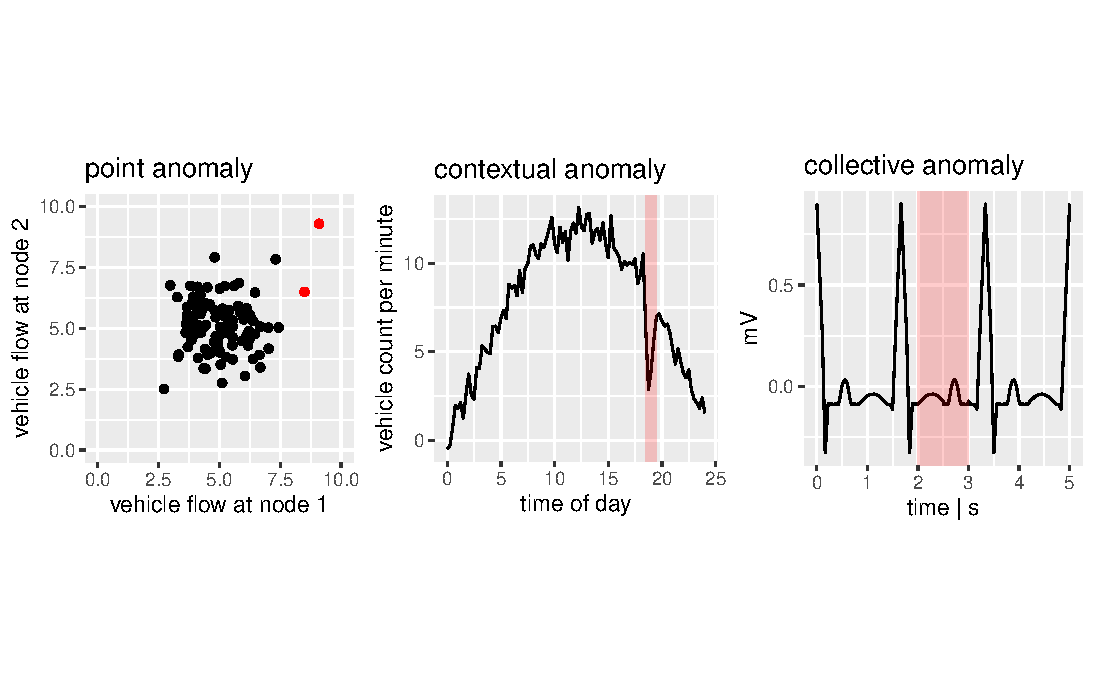
\includegraphics[width=0.9\linewidth, trim=0 75 0 75, clip]{images/types.pdf}%
% trim: [trim=left bottom right top, clip]
\caption{Examples for different types of anomalies. Anomalous data points are marked in red. Left: point anomaly. Center: contextual anomaly. Right: collective anomaly. The distinction is adapted from \cite{chandola2009anomaly}.}
\label{fig:types}
\end{figure*}


\section{Challenges of anomaly detection models} \label{sec:challenges}

Typical classification models in statistical learning or machine learning are trained with a considerable amount of training data, and it's performance is then evaluated using a separate set of test data \cite{larose2014discovering}. To solve such classification problems straightforward, it is necessary that the classes are more or less equally distributed. In a simplified anomaly detection use case, we may have a binary classification problem: normal observations vs. non-normal observations. We may face two possible scenarios:
\begin{enumerate}
    \item non-normal observations are highly underrepresented in the training data, or
    \item non-normal observations are totally absent in the training data.
\end{enumerate}

In the first scenario, the researcher in place has a picture about what is an anomaly by observing and labeling it as such. In the second scenario, the model may highlight extreme events, which then get analyzed post hoc if evaluated as meaningful. However, in real use cases there may exist a high variety of different forms of anomalies, which are either underrepresented (i.e., class imbalance \cite{dal2017credit}) or non-existent in the training data. Similarly, new types of anomalies can arise over time, for which the model was not trained on in the first place (i.e., concept drift \cite{chandola2009anomaly}). For instance, in a fraud detection framework, which is very similar to anomaly detection, the fraudsters may implement new strategies, which can not be known to the model \cite{dal2017credit}. Therefore, even if the model was trained with anomalous observations, it might not be able to generalize to new anomalies. Lastly, the entire training data may underlie a \emph{sample selection bias}, which means that only particular, conspicuous observations have been labelled in the first place \cite{dal2017credit}. This issue is not terminable, but one should be aware of its existence.

Depending on the presence of anomalies in the training data, we can deploy models of one of three categories \cite{chandola2009anomaly}:
\begin{enumerate}
    \item \emph{supervised anomaly detection}: both classes are present in the training data 
    \item \emph{semi-supervised anomaly detection}: only the normal class is represented in the training data
    \item \emph{unsupervised anomaly detection}: no training data required at all
\end{enumerate}

\section{Methods for anomaly detection}

In ordinary statistical approaches, outliers or anomalous data points are typically disruptive elements in the model building process. Originating from the motivation to handle those disruptive data points, different methods to identify and potentially drop those outliers have been established. Those are often necessary to fulfill distributional requirements on a model. In anomaly detection however, the outliers are the actual observations of interest. Therefore, one can adapt methods developed for outlier detection and use them as primary statistics of interest.

The different kinds of anomalies (see Section~\ref{sec:whatisanomaly}) require different anomaly detection methods. For instance, \emph{distance-based} approaches have been shown suitable for \emph{point anomalies}, both  \emph{distance-based} and \emph{density-based} approaches for \emph{contextual anomalies}, and \emph{density-based} approaches for \emph{collective outliers} \cite{gogoi2011survey}. In any case, the suitability strongly depends on the distribution of the data (e.g., multivariate Normal vs. uniform vs. skewed), and many other factors \cite{gogoi2011survey}. Therefore, for a given data set, suitability of a given method should be evaluated individually. 

The methods presented in the following work on numerical data. I get started with rather intuitive approaches, and continue to more specific models. 


\subsection{Distance-based methods}

\subsubsection{Static approaches}

The most intuitive approaches take some measure of central tendency, and some measure of variability of the data, such as mean and standard deviation. In this parametric approach, the data requires to follow a Normal distribution \cite{howell1998statistical}. One may classify a particular observation as anomalous, when it deviates more than 2 or 3 standard deviations from the mean of the distribution. The number of standard deviations chosen as threshold may deviate according to the specific use case. The use of a low number could lead to low specificity, i.e., a high false-positive rate, whereas the use of a high number could lead to low sensitivity, i.e., a high false-negative rate (see Section~\ref{sec:eval}).

The issue with the preceding approach is, that both mean and standard deviation are highly sensitive to outliers or anomalies \cite{leys2013detecting}, meaning that the estimation of mean and standard deviation themselves are influenced by the outlier. Therefore, the median is proposed as more robust measure of central tendency, and the median absolute deviation of the median ($MAD$) can be deployed as measure of variability. Analogous to before, an observation can be classified as anomalous if the an observation deviates more then $2$ to $3$ times from the median than the $MAD$ \cite{leys2013detecting}.

Similarly, the interquartile range ($IQR$) is commonly used to classify outliers during the creation of boxplots \cite{dawson2011significant} and denotes the distance between 1$^{st}$ and 3$^{rd}$ quartile. An outlier then is an observation, that deviates e.g. $1.5 \cdot IQR$ from the sample median.

\subsubsection{Sliding windows}

Especially for auto-correlated data as time series, a sliding window approach can be suitable to detect anomalies. The strategy is simple: a one-sided or two-sided window including $k$ neighboring data points is defined. Then, for each observation, a decision is made if the magnitude of the observation corresponds to what is expected by the neighboring observations, or if the observed data point deviates significantly from this expectation. This strategy can be suitable for a contextual anomaly as depicted in Fig.~\ref{fig:types} (center). There are a variety of possible implementations of sliding windows. One possible implementation is to calculate a prediction confidence interval ($PCI$, \cite{yu2014time}), by first predicting the data point $\hat{x}_i$ by its neighboring data points (eq.~\ref{eq:predwindow}),

\begin{equation} \label{eq:predwindow}
    \hat{x}_i = \dfrac{\sum \limits_{j=1}^k w_{i-j} x_{i-j} + \sum \limits_{j=1}^k w_{i+j} x_{i+j} }{\sum \limits_{j=1}^k w_{i-j} + \sum \limits_{j=1}^k w_{i+j}}
\end{equation}

with $k$ neighboring observations $x_{i \pm j}$ on each side, and $w_{i \pm j}$ the weighting of each neighbor, with proximal data points weighted higher than distant data points. The prediction confidence interval is then estimated via

\begin{equation} \label{eq:pci}
    PCI = \hat{x}_i \pm t_{\frac{\alpha}{2},2k-1} \cdot s \cdot \sqrt{1+\frac{1}{2k}}
\end{equation}

with $t_{\frac{\alpha}{2},2k-1}$ being the quantile of the student's t-distribution with significance level $\alpha$ and $2k-1$ degrees of freedom, and $s$ the empirical standard deviation. Lastly, it is evaluated if the $PCI$ includes the observed data point $x_i$.

\hspace{1em}

\textit{All approaches presented above operate on univariate data, or they neglect interdependencies between variables if applied to a multivariate data set. All the following approaches work on multivariate data.}

\hspace{1em}


\subsubsection{Cook's distance}

A (linear) regression model can be trained on all data points except the data point which we want to evaluate. We can then predict the data point by the model, and calculate a prediction error. If the prediction error is sufficiently high -- i.e., decided by a predefined threshold -- the data point under consideration can be classified as anomalous.

An often used implementation of this idea is the Cook's distance \cite{cook1977detection}. A Cook's distance $D_i$ can be computed for every observation $i$ and represents the sum of all changes in a regression model with observation $i$ removed, compared to the full model:

\begin{eqnarray}
    D_i = \dfrac{\sum \limits_{j=1}^n (\hat{x}_j - \hat{x}_j^{(-i)})^2 }{ps^2}
\end{eqnarray}

where $\hat{x}_j$ is the prediction of observation $i$ of the full model (trained on a total of $n$ observations), and $\hat{x}_j^{(-i)}$ of the model without observation $i$, $p$ is the number of fitted parameters (number of predictors $+1$), and $s^2$ is the mean squared error of the full regression model.
A threshold of $\frac{4}{n-p}$ may be chosen to classify a data point as anomalous, if getting exceeded \cite{rahman2012multiple}.

\subsection{Density-based methods - Local Outlier Factor (LOF)} \label{sec:lof}

%\textcolor{red}{ToDo nach Feedback von Hanno: den LOF Ansatz nochmal verständlicher schreiben, und ggfls visualisieren (Formeln, wenn es fürs Verständnis passt, reduzieren, und vielleicht nur die letzte behalten)}

Local Outlier Factor (LOF) first calculates the distance of a (multivariate) data point to its neighbors to get a local density (\cite{breunig2000lof}). The distance function applied needs particular considerations. For instance for Normally distributed data, a Euclidean distance might be sufficient, whereas for categorical data, or generally for more complex distributions, distance functions may be based on information theory or implicitly transform the underlying data \cite{cha2007comprehensive}. In a second step the fraction of local densities of the neighbors to the data points own local density is calculated. Is this fraction around $1.0$, the local density is very homogeneous. Is this fraction $>>1$, the point is either a marginal data point or a outlier. There exist further extensions of LOF-based methods, and application for fraud detection data \cite{ma2013fault} and traffic data \cite{ma2016density}. The algorithm works as follows \cite{ma2016density}, and some major quantities are visualized in Fig.~\ref{fig:lof}:

\begin{enumerate}
    \item Define $k$ and find the $k$-th nearest data points in neighborhood $K$ around point $x_i$. Calculate $kdist(x_i)$ as the distance to the $k$-th nearest data point (Fig.~\ref{fig:lof}).
    
    \item For each neighbor $x_k$  of $x_i$, and also for each other data point $x_j$, calculate its own $kdist(.)$.
        
    \item Calculate a reachability distance $rdist(.)$ between two points $x_i$ and $x_j$. This is, a reachability distance between each combination of points in the data is calculated. If the point $x_j$ is within neighborhood of $x_i$, $rdist(x_i,x_j)$ is set to be the $kdist(x_i)$. On the other hand, if the point $x_j$ is not within the neighborhood of $x_i$, then the $rdist(x_i,x_j)$ corresponds to the actual distance $dist(x_i,x_j)$ between those two data points (Fig.~\ref{fig:lof}).
    
    \item Calculate local reachability density $lrd(.)$ of data point $x_i$. This is the inverse of the average reachability distance of all neighbors $x_k$ to $x_i$.
        
        \begin{align}
            \label{eq:lrd}
            lrd(x_i) &= \dfrac{k}{\sum \limits_{x_k \in K} rdist(x_k,x_i) }%\\
            %R(m) &= \{ s | dist(m,s) < kdist(m) \} \\
            %lrd(x_i) &= \dfrac{|R(m)|}{\sum \limits_{s \in R(m)} rdist(m,s)}
        \end{align}
    
    \item Calculate $LOF$ by comparing the $lrd(.)$ of a data point $x_i$ with the $lrd$ of its neighbors $x_j$:
    
        \begin{eqnarray}
            \label{eq:lof}
            %lof(m) = \dfrac{\sum \limits_{s \in R(m)} lrd(s)}{|R(m)| \cdot  lrd(m)}
            LOF(x_i) = \dfrac{\sum \limits_{x_k \in K} lrd(x_k)}{k \cdot  lrd(x_i)}
        \end{eqnarray}
            
        
            
\end{enumerate}

\begin{figure}[t]
\centering
%\includesvg[width=0.9\linewidth]{images/lof.svg}%
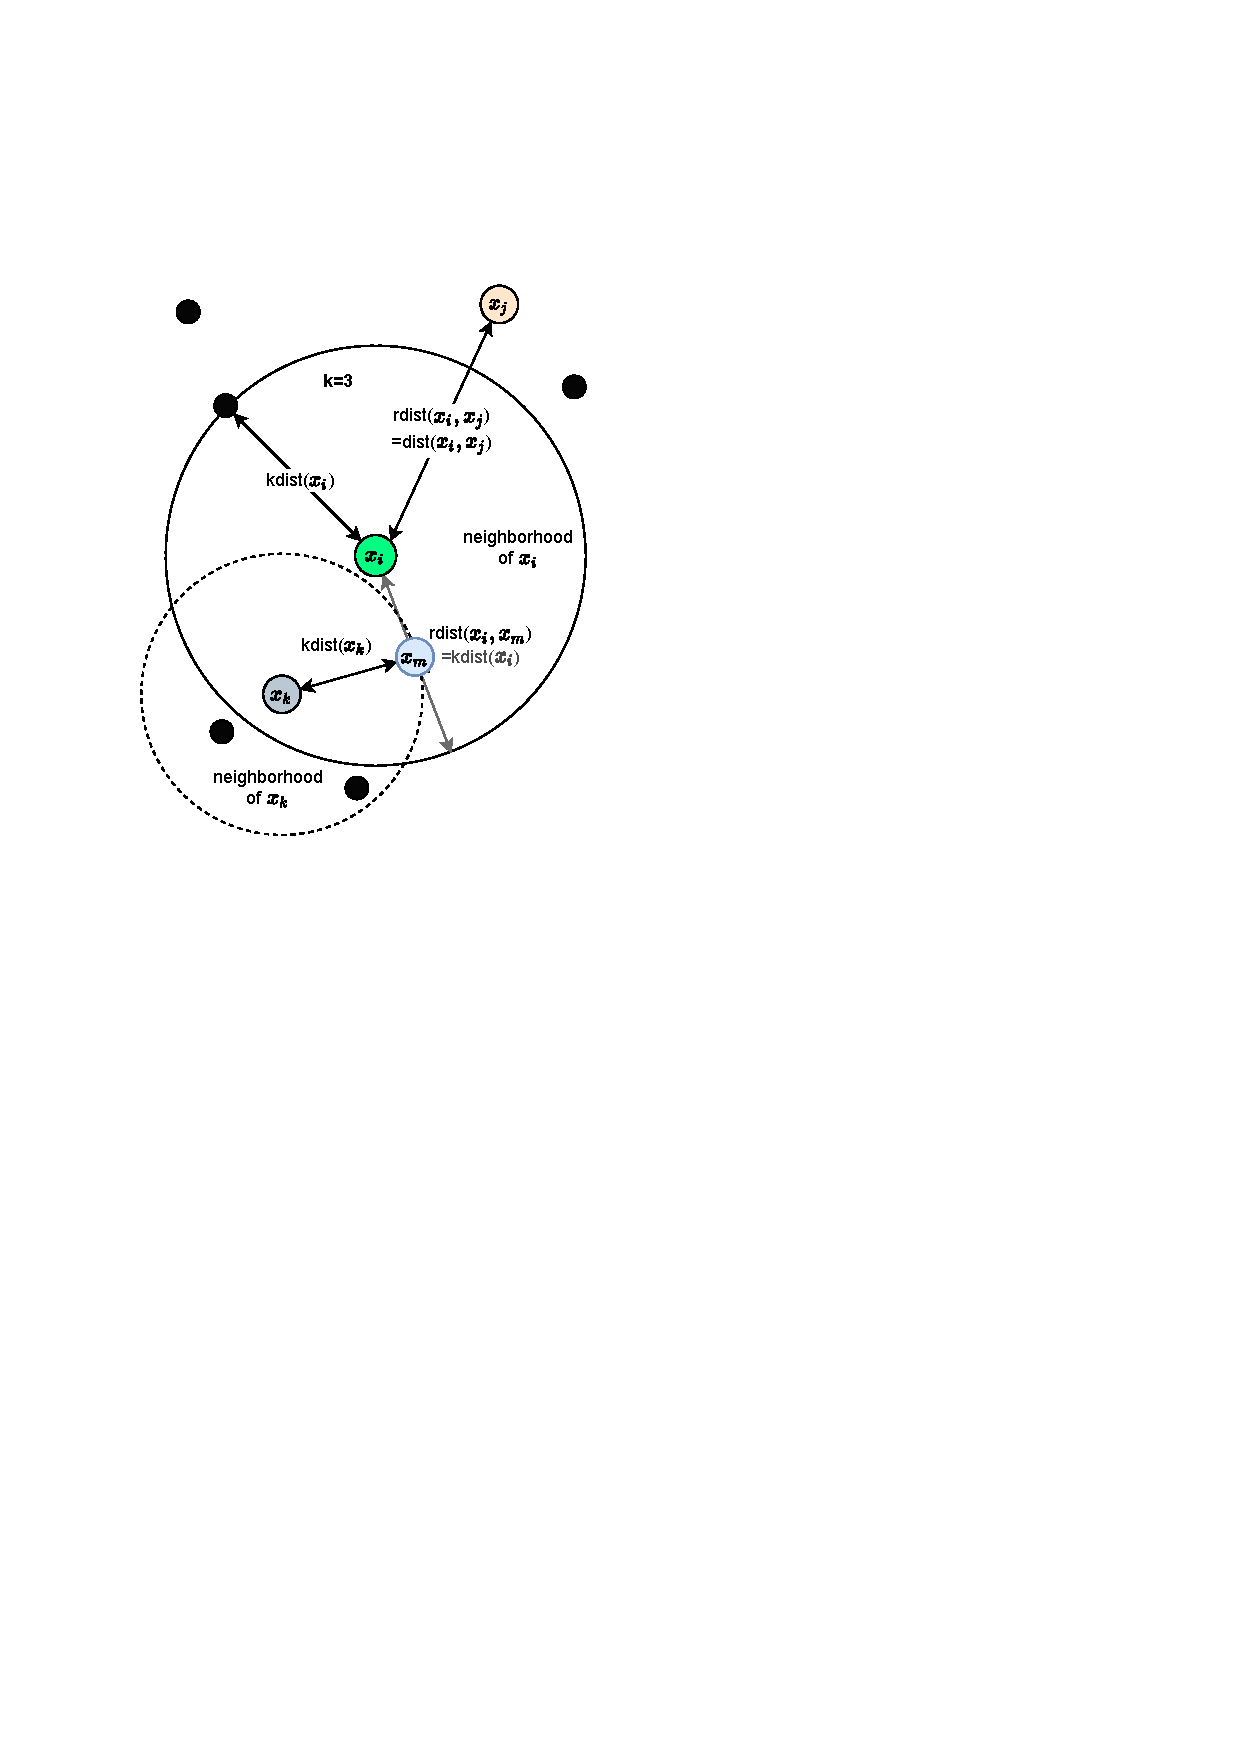
\includegraphics[page=1,width=.45\textwidth, trim=60 440 310 120, clip]{images/lof.pdf} 
% trim: [trim=left bottom right top, clip]
\caption{Metrics used for calculation of local outlier factor (LOF). All points (colored and black) represent data points in (here) two-dimensional space. The solid circle encloses the neighborhood of data point $x_i$ (green) and comprises $k=3$ other data points. The $kdist(x_i)$ is the distance to the $k=3$-rd proximal data point. Data point $x_k$ is annotated as an example for a data point within neighborhood of $x_i$. The dashed circle encloses the neighborhood of $x_k$ with radius $kdist(x_k)$. Reachability distance $rdist(.)$ of $x_i$ is illustrated to one data point $x_j$ outside its neighborhood, and to one data point $x_m$ inside its neighborhood. For data points outside the neighborhood, $rdist(x_i,x_j)$ is equal to the distance $dist(x_i,x_j)$ between the points. For data points inside the neighborhood, $rdist(x_i,x_m)$ is equal to $kdist(x_i)$. The $lrd$ of a data point is calculated using the the $rdist(.)$ of all its neighbors (eq.~\ref{eq:lrd}). Finally, the $LOF$ of a data point is calculated by comparing the average $lrd(.)$ of all neighbors to the $lrd(.)$ of a data point itself (eq.~\ref{eq:lof}).}
\label{fig:lof}
\end{figure}

LOF is therefore the average $lrd(.)$ of the neighbors, divided by the average $lrd(.)$ of the point itself. LOF-based methods are able to handle data sets with high heterogeneity of densities within the data and are also able to handle high dimensional data. Further, by the use of different distance measures (e.g., Euclidean, Manhattan, Mahalanobis, Jaccard, ...) \cite{cha2007comprehensive} it is highly flexible for different types of data.

However, depending on the degree of variability of local densities, initial consideration about a decision threshold is essential. For instance, in a highly homogeneous data set (e.g., a lattice), a $LOF$ of $1.1$ may indicate an anomaly. Contrarily, in a very heterogeneous data set, a $LOF$ of $2.0$ might still be acceptable. Notably, density-based methods need considerable more computational effort than ordinary statistical  methods, and also a bit more computational power as distance-based methods \cite{ma2016density}.

\subsection{Tree-based: Isolation Forest} \label{sec:iforests}

Particular anomaly detection methods originated from algorithms developed in a different context, but which demonstrated helpful properties with respect to anomaly detection. One such example are classification and regression trees (CART) \cite{loh2011classification}, which can be reinterpreted and used for \emph{isolation forests} \cite{liu2008isolation}.

Tree-based methods try to separate a data set in an iterative fashion.
%(Fig.~\ref{fig:itree}).
The aim is to gain data subsets -- represented in the leaves of the tree -- which are maximally homogeneous (i.e., pure), and maximally different to other data subsets (i.e., other leaves). Therefore, each fork is conducted to obtain maximal pureness in the resulting data subsets by minimizing information gain, which is quantified using e.g. entropy \cite{loh2011classification}. The rationale behind the isolation forest is, that an anomaly is easier to separate from the rest of the observations, than a normal observation is. Therefore, anomalous observations might have a higher probability of being represented in leaves, which are more proximal to the root. Normal observations however should have a higher probability being represented in leaves more distant from the root \cite{liu2008isolation}. The original implementation of isolation forests made use of random splits of the data set, and showed, that random splits are sufficient to identify outliers \cite{liu2008isolation}. However, information theory based splits -- i.e., entropy based -- lead to a more fast and robust isolation of the anomalous data points \cite{liao2018entropy}.

% \begin{figure}[t]
% \centering
% %\includesvg[width=0.9\linewidth]{images/lof.svg}%
% 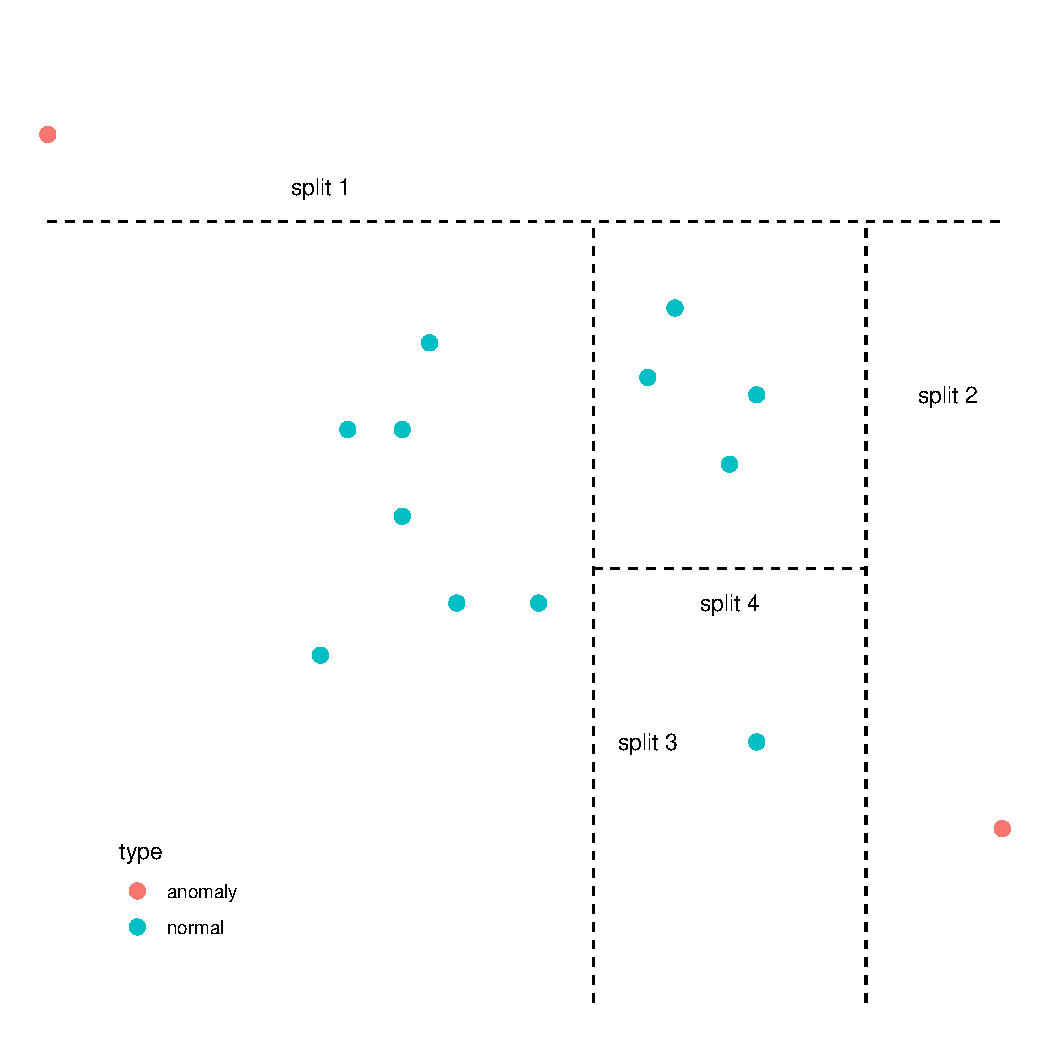
\includegraphics[page=1,width=.45\textwidth, trim=0 0 0 0, clip]{images/itree.pdf} 
% % trim: [trim=left bottom right top, clip]
% \caption{Schematic segmentation of the data space with a single isolation tree. \textcolor{red}{TODO: make nicer!} Blue data points are normal observations, whereas red data points represent anomalies. Each split (dashed line) aims to separate the data set to minimize entropy in the subset. Only 4 splits were conducted within this tree. On average, anomalies get separated earlier from normal data and are therefore represented in pure sub-spaces (i.e., leaves) after fewer splits. Path lengths of each observation is averaged across many isolation trees, with anomalies exposing shorter average path lengths than normal observations.}
% \label{fig:itree}
% \end{figure}

In isolation forests, the computation of different trees is repeated many times using different but overlapping samples of the full data set. For each observation, a metric for \textit{being anomalous} can be computed by calculating the average path length (i.e., distance from root to leave, in which the observation is located) \cite{liu2008isolation}, with short average path lengths for anomalies. The method can either be used in both a supervised, and an unsupervised fashion. Isolation forests are further proposed to be a suitable method for finding anomalies in streaming data due to relatively low computational costs \cite{mercader2020automatic}.

% to do: optional: mit formeln fuettern? zB fuer Path Length

\subsection{Network-based: Deep autoencoder} \label{sec:auto}

Due to the rise in data availability and computational power, the use and development of neural network-based techniques has experienced a "Cambrian explosion" \cite{aggarwal2018neural}. One member of the family of neural networks are autoencoders, which are frequently used in anomaly detection \cite{geron2019hands}. They further belong to the semi-supervised learning algorithms, as no labeling of the data is needed. However, the algorithms implicitly assumes the presence of exactly one particular class in the data, i.e., non-anomalies, which they are trained on. Autoencoders are frequently used to analyze image data, for instance to detect anomalous structures on medical images \cite{sato2018primitive} or to detect production defects \cite{carrera2016defect}. However, autoencoders can also be applied to different data structures such as time series \cite{zhang2019time}.


The principle is quite simple and visualized in Fig.~\ref{fig:auto}. The input data is propagated through the network. Within the network, the size of the hidden layers and therefore data dimensionality is continuously decreased (encoding unit). A bottleneck layer is situated in the center of the network. After passing the bottleneck layer, the size of the hidden layers and therefore data dimensionality is continuously increased (decoding unit) \cite{geron2019hands}. Importantly, the size of the output layer must correspond to the size of the input layer. During training, the network weights are optimized in a fashion, that the information at the output layer closely corresponds to the information at the input layer. A loss function can then be computed as the divergence between input layer and output layer. If the trained network is faced with an anomalous observation, the reconstruction should not work as expected, and the computed loss between input data and output data is higher than some predefined threshold \cite{geron2019hands,an2015variational}.

% draw with this shiny app https://alexlenail.me/NN-SVG/index.html
% todo: cite shiny app

\begin{figure}[t]
\centering
\includesvg[width=0.9\linewidth]{images/nn.svg}%
\caption{Exemplary architecture of a deep autoencoder. The raw data enters the autoencoder in the input layer (leftmost layer), and is propagated through hidden layers. The central hidden layer comprises only few neurons and is considered a bottleneck layer. The size of the hidden layers decrease in the first half, and increase in the second half of the hierarchy. Typically, the network is symmetrical. In a autoencoder which is trained with normal observations, the output layer (rightmost layer) is supposed to reconstruct the input data. Reconstruction fails (i.e., high error between input layer and output layer) for anomalous observations. Visualization created with \cite{lenail2019nn}.}
\label{fig:auto}
\end{figure}

Data transformation with autoencoders show some similarities to a principle component analysis (PCA) \cite{abdi2010principal}. In a PCA, redundant information is eliminated by creating uncorrelated features, which is accomplished by transforming the axes of the data space. The transformed data (i.e., principle components) are linear combinations of the input features. This process corresponds to the encoder unit of the deep autoencoder in Fig.~\ref{fig:auto}. Typically, the principle components which explain most part of the variation in the data are preserved, and the principle components which explain few variation in the data are discarded. These components are reflected by the few nodes of the bottleneck layer in the central of the autoencoder. Subsequently, a large proportion of the original input data can be retrieved from the information in the preserved principle components via linear combinations, which corresponds to the right half of the autoencoder in Fig.~\ref{fig:auto} (decoding unit). Due to the bottleneck layer, the output data is likely to contain less information than the original input data. However, the network is trained to reconstruct as much information as possible. It can be shown that the optimal autoencoder can be identical to a PCA \cite{geron2019hands}. However, this is only the case if the activation functions within each neuron are strictly linear, and the loss is computed using mean squared error \cite{geron2019hands}. Using non-linear activation functions -- as implemented in most neural networks \cite{rashid2016make} -- autoencoders show higher versatility than PCA.

\section{Anomaly detection vs. change detection}

Despite being closely related, there is a distinction between an anomaly detection paradigm and a change detection paradigm. Anomaly detection aims to find anomalous data points or -- within time series -- intervals of anomalous data. We thereby assume that there is a stable underlying process which generates the data we observe, and we test the plausibility of an observation with respect to the underlying process. However, the underlying process remains unchanged over time. In change detection however, we assume that the underlying process which generates the data can change. Therefore, we are faced with prolonged periods where we observe particular data points with different probabilities.
%Hence, whereas decision rules in anomaly detection paradigms are "one-shot", decision rules in change detection paradigms are sequential (REF Vortrag XX).

Picture the use case of traffic surveillance at a particular lane. Due to the set up of a construction side on a parallel lane nearby, commuters might start using this lane as response to slow traffic flow at the other lane. The activity on this lane might increase continuously for several weeks, until reaching a steady state. The underlying process which generates our observed data has changed slowly, but is now clearly distinct from the underlying process before the construction side was set up. Therefore, with the old anomaly detection model applied to the updated traffic situation, we may get a lot of observations labelled as anomalous. 

For this scenario, an operator might decide in the following ways: (i.) manually update the model, to account for the change in the generative process, (ii.) temporarily lower the sensibility of the model, e.g. by changing some threshold, (iii.) allowing the model to change auto-didactically, but alarming the operator about such a change, or (iv.) without alarming the operator.

Change detection encompasses a whole bunch of additional methods, such as \emph{changepoint detection} \cite{tartakovsky2012efficient}, and is outside the scope of the present work.
Recalling two major problems in anomaly detection paradigm (Section~\ref{sec:challenges}): class imbalance, and context drift, we learned that all proposed anomaly detection algorithms are in particular designed to handle imbalanced classes. However, context drifts can often be handled using change detection paradigms.  

\section{Evaluation of anomaly detection} \label{sec:eval}

Having built one or multiple potential anomaly detection algorithms, we are interested in their performance to evaluate their operational readiness. Therefore, we predict labelled test observations by the model. We subdivide predicted observations in true positives $TP$ (anomaly correctly detected), false positives $FP$ (anomaly detected, whereas observation is actually normal), true negatives $TN$ (normal observation correctly classified as normal), and false negatives $FN$ (anomaly incorrectly classified as normal).  We quantify performance, e.g. via their true positive rate $TPR$, i.e., sensitivity:

\begin{eqnarray} \label{eq:tpr}
    TPR = \dfrac{ \text{TP} }{ \text{TP}+\text{FP} }
\end{eqnarray}

and similarly in their false positive rate $FPR$, equivalent to $1-\text{specificity}$:

\begin{eqnarray}  \label{eq:fpr}
    FPR = \dfrac{ \text{FP} }{ \text{FP}+\text{TN} }
\end{eqnarray}

We might also look at indicators which combine those two measures, such as $accuracy$ or $F1$-score, with "ideal" detectors converge to scores around $1$:

\begin{align}  \label{eq:accuracy}
    accuracy &= \dfrac{ \text{TP+TN} }{ \text{TP+FP+TN+FN} } \\
    F1 &= \dfrac{ 2 \cdot \text{TP}  } {  2 \cdot \text{TP+FP+FN}  }
\end{align}

By adjusting the decision threshold for an anomaly, we must find a trade-off between $TPR$ and $FPR$. One possibility is to plot those quantities for diverse thresholds in a receiver operating characteristic ($ROC$) curve \cite{bewick2004statistics}, which is exemplary shown in Fig.~\ref{fig:roc}. The area under the curve ($AUC$) can be used as general performance criterion, with values around $0.5$ representing models which perform by pure chance, and values converging to $1$ representing "ideal" detectors.

\begin{figure}[t]
\centering
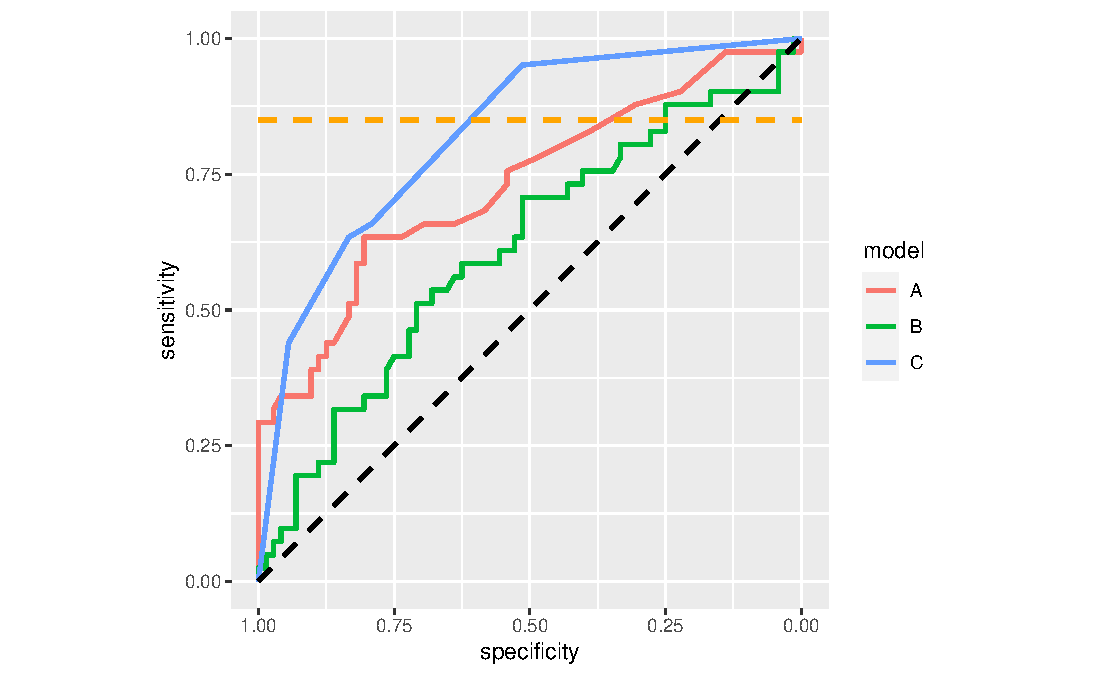
\includegraphics[width=0.95\linewidth, trim=65 0 65 0, clip]{images/ROC.pdf}%
\caption{Receiver operator characteristic (ROC) \cite{bewick2004statistics} curve for artificial anomaly detection models. The underlying data is simulated. $Sensitivity$ to anomalous observations (i.e., $TPR$) is plotted against $1-Specificity$ (i.e., $FPR$). The area under the curve (AUC) indicates model performance. AUC converges to $0.5$ for models which perform to pure chance (black dashed line), or to $1$ for "optimal" models. The blue, red, and green lines indicate the behavior of $TPR$ versus $FPR$ for different decision thresholds applied to the respective models. The orange dashed line indicates a decision boundary on the sensitivity. If the demands on a model are to detect $85\%$ of anomalies, one may decide for a model which has a low $FPR$ (i.e., high $specificity$) along this boundary. Model C (blue) would fulfill this criterion and performs better than the competing models with highest AUC.}
\label{fig:roc}
\end{figure}



%ICPR poster für Inspiration
% https://www.underline.io/events/69/posters/1945/poster/11617-1689---evaluation-of-anomaly-detection-algorithms-for-the-real-world-applications

%Etwas diskutieren, was für Evaluierungsmetriken verwendet werden können (i.e., AUC-ROC)


\section{Applications for city traffic data}

In this section, I will discuss studies which deployed some of the above methods for anomaly detection in the context of urban traffic data. By purpose, the following studies were chosen to be based on different use cases and different kinds of data. With this heterogeneity, the diversity of possible use cases shall be reflected. I will not report a study using distance-based approaches, because they are supposed to be outperformed by other approaches \cite{chen2010comparison}. However, I will investigate on studies using density-based (LOF, Section~\ref{sec:lof}), tree-based (isolation forests, Section~\ref{sec:iforests}), and network-based approaches (deep autoencoders, Section~\ref{sec:auto}). Despite having used different anomaly detection models in the following studies, all models are meant to be transferable to the respective other studies, with merely minor adjustments in the model design.   

\subsection{Density-based Outlier Detection by Local Outlier Factor on Large-scale Traffic Data \cite{ma2016density}}
\label{sec:ex1}

The study of Ma and colleagues focused on data from one 4-arm junction. At this junction, vehicles were counted minute-wise and added to three variables: one variable decoding the direction of arrival (4 possibilities), one variable decoding the direction of departure (4 possibilities), and one variable decoding the combination of those two (11 possibilities, from one particular lane cars were not allowed to turn left). They analyzed those count data over a time interval of 3 hours each. For each traffic cycle (i.e., a green period of a particular entry point) the vehicles passing were counted and the counts distributed to those 19 directional variables. The counts were produced by manually observing raw video data. Each traffic cycle was further manually labelled as normal or anomalous. The observers classified a traffic cycle as anomaly, if (i.) hardware failed, (ii.) repeated jams in entry or exit point were discovered, (iii.) vehicles obstructed an entry or exit point, (iv.) a low volume in an entry/exit was observed, or (v.) jams in an entry/exit caused low volume in a different entry/exit \cite{ngan2015outlier}. They analyzed 46 sessions in total, and separately analyzed the morning rush hour periods (23 sessions) and the evening rush hour period (23 sessions). To reduce data dimensionality, they started with a PCA (Section~\ref{sec:auto}) for each of the 19 variables separately over the traffic cycles ($>80$ cycles per variable) and maintained the two first components per variable. Each transformed data point now represented a two-dimensional projection from an entire 3~hours traffic observation. Anomalies where then detected using the LOF algorithm as outlined in Section~\ref{sec:lof} with a neighborhood of $k=7$. They reported an accuracy (cf. eq.~\ref{eq:accuracy}) of $92\%$ and $95\%$ for their data sets (morning vs. evening, respectively). However, their high accuracy is a bit white-washed. A baseline model by itself -- a simplest possible model, which would only predicting non-anomalies -- would yield an accuracy far above $50\%$ in such an unbalanced data set. Furthermore, their $TPR$ (cf. eq.~\ref{eq:tpr}) was only $6\%$ and $29\%$ in their data sets.
 
In summary, the researchers used an interesting and promising approach. However, performance of their models is still not suitable for an operational scenario.


\subsection{Automatic incident detection on freeways based on Bluetooth traffic monitoring \cite{mercader2020automatic}}
\label{sec:ex2}

Mercader \& Haddad \cite{mercader2020automatic} predicted anomalies in different road segments using isolation forests (Section~\ref{sec:iforests}). Despite the analysis being based on data retrieved from a highway, the method can likewise be used to predict anomalies in urban traffic or pedestrian zones, which will likely be accompanied with higher dimensional data.

Aforesaid highway had several measurement stations which collected the MAC addresses and time stamps of each passing cars' Bluetooth devices. Using the differences in time stamps of the respective MAC addresses between two stations (corresponding to one road segment), it was possible to calculate the direction of an individual vehicle and an average vehicle velocity for the road segment. The velocity and directional data then was discretized into intervals of 5 minutes each. For each time bin, the following features have been engineered:
\begin{enumerate}
    \item time of day (discretized interval)
    \item average velocity
    \item relative change of velocity with respect to previous time interval
    \item relative change of velocity with respect to upstream segment
    \item relative change of velocity with respect to downstream segment
    \item relative change of velocity with respect to upstream segment in the previous time bin
    \item relative change of velocity with respect to downstream segment in the previous time bin
\end{enumerate}

Those 7 features were used to predict the respective traffic state in a particular segment. For each segment, a separate isolation forest was grown. The segments at the border were not modelled explicitly, because not all of the features \#4 to \#7 could be engineered for border segments. They authors used the original implementation of isolation forests (Section~\ref{sec:iforests}), which deploys random splits to subdivide the data sets instead of entropy.

The authors analyzed a data set encompassing 90 days, of which they used 83 days for training and 7 days for model evaluation. Isolation forests in this context operate in an semi-supervised fashion. Therefore, the training data was not labelled. The authors merely labelled the 7 days of test data, by analyzing incidence reports of the traffic control center, and manually comparing the reports with the raw data. Therefore, each road segment and time bin in the test data was hand-labelled as normal or anomaly. 

They varied two hyperparameters in the isolation forest, (i.) the number of trees in the network, and (ii.) the size of the random sub-samples, used to train the different trees, and (iii.) the detection threshold, i.e. which proportion of the data with shortest average path lengths shall be classified as anomalous. Firstly, they found that the forests were rather insensitive to changes in hyperparameters (i.) and (ii.). Secondly, using varying detection thresholds (i.e., hyperparameter (iii.)), they found that isolation forests for the different road segments exceeded AUC values between 0.9797 and 0.9987 (Md.~0.9977) in all road segments (cf. Section~\ref{fig:roc}). Even at the segment with worst performance (AUC of 0.9797), at a particular detection threshold, the algorithm detected 90\% of the incidents (i.e., TPR), with a FPR of only 1.5\%. Translated to a operating environment with this model in place and a time binning of 5 minutes, an operator which supervises the alarms of the model would encounter a false positive detection on average every 5.5 hours for this segment. 
%berechnet als erwartungswert der geometrischen verteilung 1/0.015*5/60
For other segments with higher AUC, this false alarms should be much scarcer.

% rausgelassen fuer jetzt: die Feature Importance.
% ist zwar interessant, weiss aber noch nicht ob ich sie brauche

In summary, the isolation forest approach yielded excellent anomaly recognition accuracy, with high TPR and low FPR.

\subsection{Autoencoders - not just anomaly detection}

Autoencoders are powerful tools for anomaly detection in a variety of use cases (Section~\ref{sec:auto}). The vanilla type of autoencoders was outlined above and operates with a encoder and an decoder module (\ref{fig:auto}). The anomaly in a vanilla autoencoder is detected by applying some threshold on the reconstruction error on the output layer. To the best of my knowledge, there is no study applying this vanilla autoencoder to traffic data. Instead, some studies translated the anomaly detection problem into a regression problem, by combining an autoencoder with a prediction model (here: also neural networks). The roles of the autoencoders in those studies was not merely anomaly detection, but feature extraction. However, because the use cases closely relate to the present research question, I will cast a glance at those studies in the following. Further, because it is a prediction problem, I will not elaborate on model performances -- which were all acceptable according to the respective authors \cite{zhang2019deep, boquet2020variational} -- but rather outline the concepts of the approach.

\subsubsection{Deep Autoencoder Neural Networks for Short-Term Traffic Congestion Prediction of Transportation Networks \cite{zhang2019deep}}
\label{sec:ex3}

Zhang and colleagues \cite{zhang2019deep} used a deep autoencoder in combination with another simple neural network to predict future road congestion status. This study deliberately differs from the preceding studies in some aspects: First, it is not pure anomaly detection with a binary outcome, but a anomaly detection algorithm is immediately combined with a prediction model to anticipate future congestion levels. Second, the model considers many preceding data points to predict future states, therefore the method needs to handle data which has more properties of time series, such as autocorrelation. Third, the input features are high dimensional, as the congestion level is predicted for several segments of the whole city of Seattle in \textit{one} unified model instead of separate models for separate segments as in example study~2 (Section~\ref{sec:ex2}).
%However, only one single model is used, instead of different parallel models for different segments, such in example study~2 (Section~\ref{sec:ex2}).    

\begin{figure}[t]
\centering
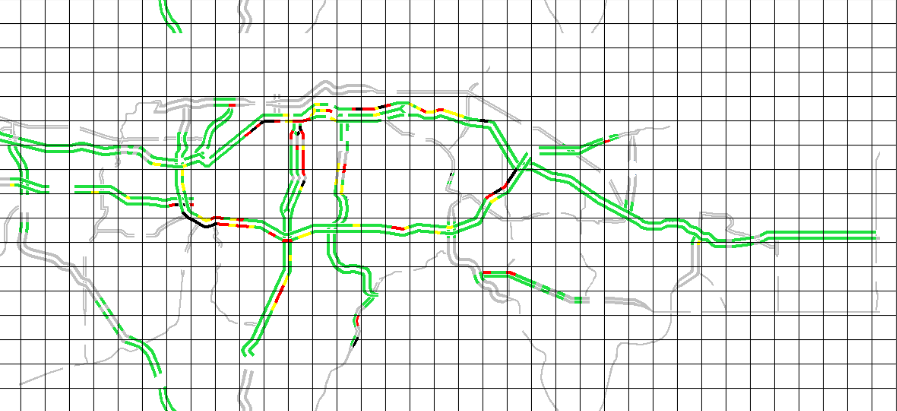
\includegraphics[width=.45\textwidth, trim=0 0 0 0, clip]{images/roads.png} 
% trim: [trim=left bottom right top, clip]
\caption{Map of traffic loading, used as input data in the autoencoder. Figure adapted from \cite{zhang2019deep}. The two-dimensional image is segmented into tiles. Traffic loading in roads is visualized with colors, from green (wide open), over yellow (moderate), red (heavy) to black (stop \& go). Average loading per tile serves as input data in the autoencoder. The map is ought to be interchangeable. Therefore this model can be trained with any comparable map, retrieved by a variety of data sources.}
\label{fig:roads}
\end{figure}


The authors proposed a rather generic method which can be applied to maps retrieved from traffic surveillance databases, such as from Google Maps or similar (Fig.~\ref{fig:roads}). Therefore, they used a two dimensional map of the city of Seattle, which -- in this analysis -- focused on data from larger highways. The map was segmented into tiles. For each tile an average traffic load was calculated and normalized. Non-road parts of each tile were neglected. Such a map is retrieved for each interval of 10~minutes. Each tile served as one input node in an autoencoder.

The authors' intuition behind the usage of autoencoders slightly differed from the primary principle of autoencoders as described in Section~\ref{sec:auto}. Instead of training the autoencoder to reconstruct the inputs of the autoencoder at the output layer, it is the future state of the input that ought to be reconstructed, or rather say predicted. To take into consideration temporal dependencies, they used not just one particular input image, but 11 input images which together covered a time period of almost 2 hours. The resulting features were put into an autoencoder with similar architecture than in Fig.~\ref{fig:auto}, but comprising far more neurons. The input layer was replicated 11 times to account for the multiple time points entering the autoencoder. The output layer was appended with two fully connected layers and an interposed dropout layer to tackle overfitting. The resulting predictions about the future traffic loads were finally reshaped into a two dimensional map.

The study adapted a method of anomaly detection to solve a prediction problem. However, in the use case of anomaly detection in urban traffic, where the anomaly can be a traffic congestion, it might be desirable to predict a future anomaly rather than detect a present anomaly. %For those reasons, this study is included in the present work.

%Data for one year was used for training (only few hours of rush hours per day), and some months of the following year for testing. Due to the fact, that the outcome is not a binary measure (anomaly vs. normal observation), but rather a continuous traffic load prediction, the evaluation metrics in this study differed. The authors used mean absolute errors amongst others to evaluate the model.

%XXX weiter und genaue Vorhersagekraft erläutern


%Table mit Vor und Nachteilen, und mögliche Datengrundlage der jeweiligen Methoden im Bezug auf Traffic, möglichen Arten der Anomalien die detektiert werden können (u.a. point / contextual / collective) + arten von training data / arten von learning (super, semi-super, unsupervised) + was für einen Wert gibt die Methode zurück (binär oder probability) + evtl (für nächstes Kapitel) Evaluation von Spec/Sens


\subsubsection{A variational autoencoder solution for road traffic forecasting systems: Missing data imputation, dimension reduction, model selection and anomaly detection \cite{boquet2020variational}}
\label{sec:ex4}

A recent study of Boquet and colleagues \cite{boquet2020variational} comprises a comprehensive analysis pipeline for traffic forecasting. Here, I will highlight some major aspects. As in the previous example study (Section~\ref{sec:ex3}), the autoencoder \textit{per se} was not used for anomaly detection. However, its functionality for reduction of data dimensionality was used (see Section~\ref{sec:auto}). The autoencoder still persisted of an encoder and a decoder part. The output layer was still optimized to reconstruct the input data. Further, they used the decoder for missing data imputation. Most importantly, the prediction model was built on the features encoded in the bottleneck layer (i.e., latent space). Therefore, the autoencoders structure elegantly led to smaller input data dimensionality in downstream prediction models. They authors applied the autoencoder and a fully connected neural network as prediction model, to real traffic data sets for the purpose of traffic forecasting, which exceeded good performance \cite{boquet2020variational}.


\section{Applicability and future directions}

In the preceding sections, several anomaly detection methods were introduced and some exemplary studies using anomaly detection for traffic data were presented. For the curse of this overview, the data foundation of the first two examples were chosen to be rather simple (Section~\ref{sec:ex1} \& Section~\ref{sec:ex2}). The methods applied in those studies -- either LOF or isolation forests -- are widely used for anomaly detection in different use cases (see Section~\ref{sec:lof} \& Section~\ref{sec:iforests}). The last two examples (Section~\ref{sec:ex3} \& Section~\ref{sec:ex4}) are based on a higher dimensional data foundation. These examples used autoencoders as one crucial step in the analysis. However, their usage of autoencoders differed from the vanilla example of autoencoders -- such as explained in Section~\ref{sec:auto}. Whereas example study~4 directly used the compressed features for subsequent prediction, example study~3 used the decompressed features for the prediction of the future state.

To decide, which modeling type is suitable for a particular use case, several thoughts have to be taken into account. First, data dimensionality. In a high dimensional data set, especially where the number of features exceeds the number of observations, feature reduction for instance via PCA or the encoder part of an autoencoder (Section~\ref{sec:auto}), similar to example studies~1 and 3. Further, autoencoders are generally well suited for high-dimensional data, whereas e.g. pure distance-based, density-based or tree-based methods may quickly run into overfitting.

Second, computational complexity. In a real-time use case, it may be desired to work with computationally efficient algorithms. If the algorithm is already trained when starting anomaly detection, supervised or semi-supervised methods such as classifiers and autoencoders, respectively, just need to predict the data. In many unsupervised models, such as LOF or isolation forests, model training and subsequent data point evaluation needs to be conducted for every new data point. With high dimensional data and a high sampling frequency, the computational time and effort might constitute a liability.

Third, the interpretability of the model. More simple models, such as statistical models or density-based models, but also isolation trees, can be interpreted by several model parameters. If the reasons for some observations being classified as anomalies are of interest -- e.g., to find the cause of the anomaly to prevent it in a long term  -- more simple models can be advantageous. However, the trend is towards more complex models, such as neural networks and autoencoders, which seem to exhibit overall high flexibility and prediction accuracy, not just in anomaly detection but in many domains.

Finally, requirements on sensitivity and specificity. As we have seen in the exemplary calculation within study~2, a good algorithm can still produce many false positive detections. If all detections undergo manual supervision, an algorithm's specificity must be sufficiently high in order to render the amount of manually supervised detections manageable. More importantly, if a detection shall be immediately transferred into action -- e.g., by sending fire brigade -- false positives would be associated with enormous costs. Consequently, a precise trade-off between sensitivity and specificity needs to be made.

A general attempt to enhance both sensitivity and specificity are ensemble learners \cite{sagi2018ensemble}. Ensemble learners either combine multiple versions of a particular model, or they combine several distinct models. One such ensemble learner in the supervised domain is Adaboost \cite{freund1996experiments}. Adaboost sequentially concatenates several prediction models, whereas the subsequent model primarily processes the observation for which the preceding model showed high uncertainty in classification. The resulting ensemble demonstrates higher sensitivity and specificity than a solitary model \cite{freund1996experiments}. Similarly, different model types (e.g., one LOF model, one PCI model, and one isolation tree) can be combined to a voting classifier \cite{sagi2018ensemble}. Each model then predicts a class for an observation, and the majority of votes will decide for the class of the observation. Voting classifiers have been shown to increase sensitivity and specificity of the predictions \cite{sagi2018ensemble}. Adjusting their threshold for class assignment, i.e., not relying on simple majority, opens many degrees of freedom for further adjustments regarding sensitivity and specificity, for instance by weighting models differently and adjusting decision thresholds for the ensemble. Further, new, specialized models for particular kinds of anomalies may be added to the ensemble within an operating environment. However, such an approach is only feasible, if the computational effort and data sampling rate is sufficiently low.

\section{Conclusion}

Within the present work I have introduced several established methods for anomaly detection. Further, I have touched upon some use cases, with a very heterogeneous data foundation, using implementations of the proposed methods in the context of urban traffic. Whereas a global trend points towards network-based methods, the decision of a particular model highly depends on the data foundation and other requirements of the particular use case. However, anomaly detection in urban traffic in general seems to work well with many types of models and data foundations. For modeling the smart city, such anomaly detection methods for urban traffic data are suitable or, rather essential, to prevent the traffic itself as well as downstream infrastructures to be get harmed by different types of malicious events.


\textcolor{red}{Bibliography: there are lots of inconsistencies in bibliography... needs to be corrected}

\printbibliography
%\begin{thebibliography}{1}

%\bibitem{Mohammadi2017}
%N. Mohammadi and J. E. Taylor, "Smart city digital twins," 2017 IEEE Symposium Series on Computational Intelligence (SSCI), Honolulu, HI, 2017, pp. 1-5, doi: 10.1109/SSCI.2017.8285439.

%\bibitem{Ouyang2014}


%\end{thebibliography}






% An example of a floating figure using the graphicx package.
% Note that \label must occur AFTER (or within) \caption.
% For figures, \caption should occur after the \includegraphics.
% Note that IEEEtran v1.7 and later has special internal code that
% is designed to preserve the operation of \label within \caption
% even when the captionsoff option is in effect. However, because
% of issues like this, it may be the safest practice to put all your
% \label just after \caption rather than within \caption{}.
%
% Reminder: the "draftcls" or "draftclsnofoot", not "draft", class
% option should be used if it is desired that the figures are to be
% displayed while in draft mode.
%
%\begin{figure}[!t]
%\centering
%\includegraphics[width=2.5in]{myfigure}
% where an .eps filename suffix will be assumed under latex, 
% and a .pdf suffix will be assumed for pdflatex; or what has been declared
% via \DeclareGraphicsExtensions.
%\caption{Simulation results for the network.}
%\label{fig_sim}
%\end{figure}

% Note that the IEEE typically puts floats only at the top, even when this
% results in a large percentage of a column being occupied by floats.


% An example of a double column floating figure using two subfigures.
% (The subfig.sty package must be loaded for this to work.)
% The subfigure \label commands are set within each subfloat command,
% and the \label for the overall figure must come after \caption.
% \hfil is used as a separator to get equal spacing.
% Watch out that the combined width of all the subfigures on a 
% line do not exceed the text width or a line break will occur.
%
%\begin{figure*}[!t]
%\centering
%\subfloat[Case I]{\includegraphics[width=2.5in]{box}%
%\label{fig_first_case}}
%\hfil
%\subfloat[Case II]{\includegraphics[width=2.5in]{box}%
%\label{fig_second_case}}
%\caption{Simulation results for the network.}
%\label{fig_sim}
%\end{figure*}
%
% Note that often IEEE papers with subfigures do not employ subfigure
% captions (using the optional argument to \subfloat[]), but instead will
% reference/describe all of them (a), (b), etc., within the main caption.
% Be aware that for subfig.sty to generate the (a), (b), etc., subfigure
% labels, the optional argument to \subfloat must be present. If a
% subcaption is not desired, just leave its contents blank,
% e.g., \subfloat[].


% An example of a floating table. Note that, for IEEE style tables, the
% \caption command should come BEFORE the table and, given that table
% captions serve much like titles, are usually capitalized except for words
% such as a, an, and, as, at, but, by, for, in, nor, of, on, or, the, to
% and up, which are usually not capitalized unless they are the first or
% last word of the caption. Table text will default to \footnotesize as
% the IEEE normally uses this smaller font for tables.
% The \label must come after \caption as always.
%
%\begin{table}[!t]
%% increase table row spacing, adjust to taste
%\renewcommand{\arraystretch}{1.3}
% if using array.sty, it might be a good idea to tweak the value of
% \extrarowheight as needed to properly center the text within the cells
%\caption{An Example of a Table}
%\label{table_example}
%\centering
%% Some packages, such as MDW tools, offer better commands for making tables
%% than the plain LaTeX2e tabular which is used here.
%\begin{tabular}{|c||c|}
%\hline
%One & Two\\
%\hline
%Three & Four\\
%\hline
%\end{tabular}
%\end{table}


% Note that the IEEE does not put floats in the very first column
% - or typically anywhere on the first page for that matter. Also,
% in-text middle ("here") positioning is typically not used, but it
% is allowed and encouraged for Computer Society conferences (but
% not Computer Society journals). Most IEEE journals/conferences use
% top floats exclusively. 
% Note that, LaTeX2e, unlike IEEE journals/conferences, places
% footnotes above bottom floats. This can be corrected via the
% \fnbelowfloat command of the stfloats package.



% trigger a \newpage just before the given reference
% number - used to balance the columns on the last page
% adjust value as needed - may need to be readjusted if
% the document is modified later
%\IEEEtriggeratref{8}
% The "triggered" command can be changed if desired:
%\IEEEtriggercmd{\enlargethispage{-5in}}

% references section

% can use a bibliography generated by BibTeX as a .bbl file
% BibTeX documentation can be easily obtained at:
% http://mirror.ctan.org/biblio/bibtex/contrib/doc/
% The IEEEtran BibTeX style support page is at:
% http://www.michaelshell.org/tex/ieeetran/bibtex/
%\bibliographystyle{IEEEtran}
% argument is your BibTeX string definitions and bibliography database(s)
%\bibliography{IEEEabrv,../bib/paper}
%
% <OR> manually copy in the resultant .bbl file
% set second argument of \begin to the number of references
% (used to reserve space for the reference number labels box)





% that's all folks
\end{document}


